\chapter{Evaluation and Results} \label{chap:evaluation}
%One liability of image-based rendering systems is the lack of a consistent  framework within which to judge the validity of the results. plenoptic modeling: an image-based rendering system mcmillan
Unfortunately, there are no publicly available benchmarks for 360\degree image synthesis with two degrees of freedom without 3D geometry, as not many methods exist that try to achieve this. Since the approach presented in Chapter~\ref{chap:implementation} is a first, basic attempt at solving this problem, this chapter presents a basic evaluation of the algorithm, based on mathematically calculable error metrics. These metrics measure the accuracy of a synthesized image compared to the ground truth and are used to assess the effect of a limited number of parameters.
%Furthermore, it compares the results of regular blending, flow-based blending, and a naive baseline algorithm to analyze whether, and in which cases an improvement could be achieved.

First, possible parameters are discussed (Section~\ref{sec:params}), followed by the presentation of the evaluation methodology (Section~\ref{sec:eval_methodology}). Then a limit evaluation is performed on virtually generated scenes to explore the limits of the algorithm in a controlled environment (Section~\ref{sec:limit_eval}). Based on the knowledge gained in the limit evaluation, a proof-of-concept evaluation is performed on real scenes (Section~\ref{sec:pof_eval}). Finally, the aggregate evaluation findings are discussed (Section~\ref{sec:discussion}).

%First the evaluation methodology is presented, outlining how the effects of a parameter are measured and evaluated. Then, the limits of the algorithm are explored using virtual scenes. With the information gleaned from this limit evaluation, the parameters are chosen for a proof-of-concept evaluation using real scenes. The results and limitations are then discussed\ldots

%- what is a scenario what is a scene
%- not performance
%- konkreter
%- wie gut koennen szenen synthetisiert werden
%- scope: basic evaluation of mathematically measurable values (no human perception)
%- these datasets could be used in the future to compare different algorithms

\section{Parameters} \label{sec:params}
Before defining the parameters to test in the limitation and proof-of-concept evaluations, this section gives an overview of possible parameters in the context of the 2DoF algorithm presented in Chapter~\ref{chap:implementation}.
The 2DoF algorithm already makes a few assumptions, for example the constraint to the viewpoint plane, the fact that the scene is static, and more (stated in Section \ref{sec:approach} on page \pageref{sec:approach}). These assumptions are upheld in the evaluation, as they are prerequisite to the function of the algorithm.

The remaining parameters (that are not constrained by the assumptions) can be divided into two categories: 
\begin{description}
    \item [Internal parameters] i.e.\ based within the algorithm, such as the blending type and the selection of input viewpoints
    \item [External parameters] i.e.\ based on the properties of the captured scene, such as the viewpoint density, or the geometry of the scene.
\end{description}      

The internal parameters can be modified after the scene has been captured, the external ones cannot.  The most prominent internal parameters based on the implementation from Chapter~\ref{chap:implementation} are:

\begin{itemize}
  \item the location of synthesized points within the scene (near walls, objects, etc)
  \item the location of synthesized points relative to the captured points
  \item the blending type, i.e.\ flow-based blending or deviation-angle-based knn blending (``regular blending'')
%  \item the selection of input viewpoints from the available captured viewpoints
  \item the optical flow algorithm used for flow-based blending
\end{itemize}

There are more internal parameters that could theoretically be modified, such as the knn blending function (the inverse sigmoid function on page~\pageref{eq:sigmoid}), or the method of approximation for 2DoF in flow-based blending (page~\pageref{subsec:2dof_flow-based}), but these will be assumed immutable for this evaluation, as the variation of these parameters would require developing new functions, which would be outside the scope of this thesis.

As for the possible external parameters, the number of different possible scenes is infinite, but the assumed key parameters are:
\begin{itemize}
  \item type of scene (outdoor, indoor, etc) \ar size and shape of scene
  \item objects within the scene
  \item density of captured viewpoints
  \item distribution of captured viewpoints
\end{itemize}

External parameters such as the camera settings (e.g. aperture, shutter speed, white balance) and the lighting throughout the scene are not considered; it is assumed that all the captures have the same camera settings and the white balance is comparable throughout the scene. Furthermore, the evaluation is restricted to indoor scenes of approximately $25m^2$. This reduces the parameter space significantly, since the fact that indoor scenes tend to be enclosed by walls enforces a maximal distance of objects to the camera.

The evaluation presented in this thesis aims to examine the effects of a few select internal and external parameters, instead of exhaustively examining all of them. In order to do this, a \emph{scenario} is designed for each selected parameter that attempts to demonstrate the effect of this parameter on the accuracy of the result. Limiting the evaluation to specific scenarios reduces the testing space but might also lead to missing some interactions between parameters. This is acceptable, since the evaluation does not aim to be comprehensive. 

%The scenario definition is the first step of the evaluation process which is presented in the next section.
%The parameters to be evaluated, along with their corresponding scenarios depend on the type of evaluation

\section{Evaluation Methodology} \label{sec:eval_methodology}
The evaluation is divided into two distinct phases: an evaluation of limits using virtual scenes, and a proof-of-concept evaluation using real scenes. Both evaluations follow the methodology depicted in Figure~\ref{fig:eval-methodology}, and consist of four steps: \emph{scenario definition}, where a scenario is designed to exemplify the parameter to test, \emph{synthesis}, where the synthesized images are calculated using the 2DoF synthesis presented in Chapter~\ref{chap:implementation}, \emph{error calculation}, where the accuracy of the synthesized images is measured, and \emph{result analysis}, where the the cause and effect of the parameters is examined. The details of these steps are described in the following sections.

\begin{figure}
		\centering
		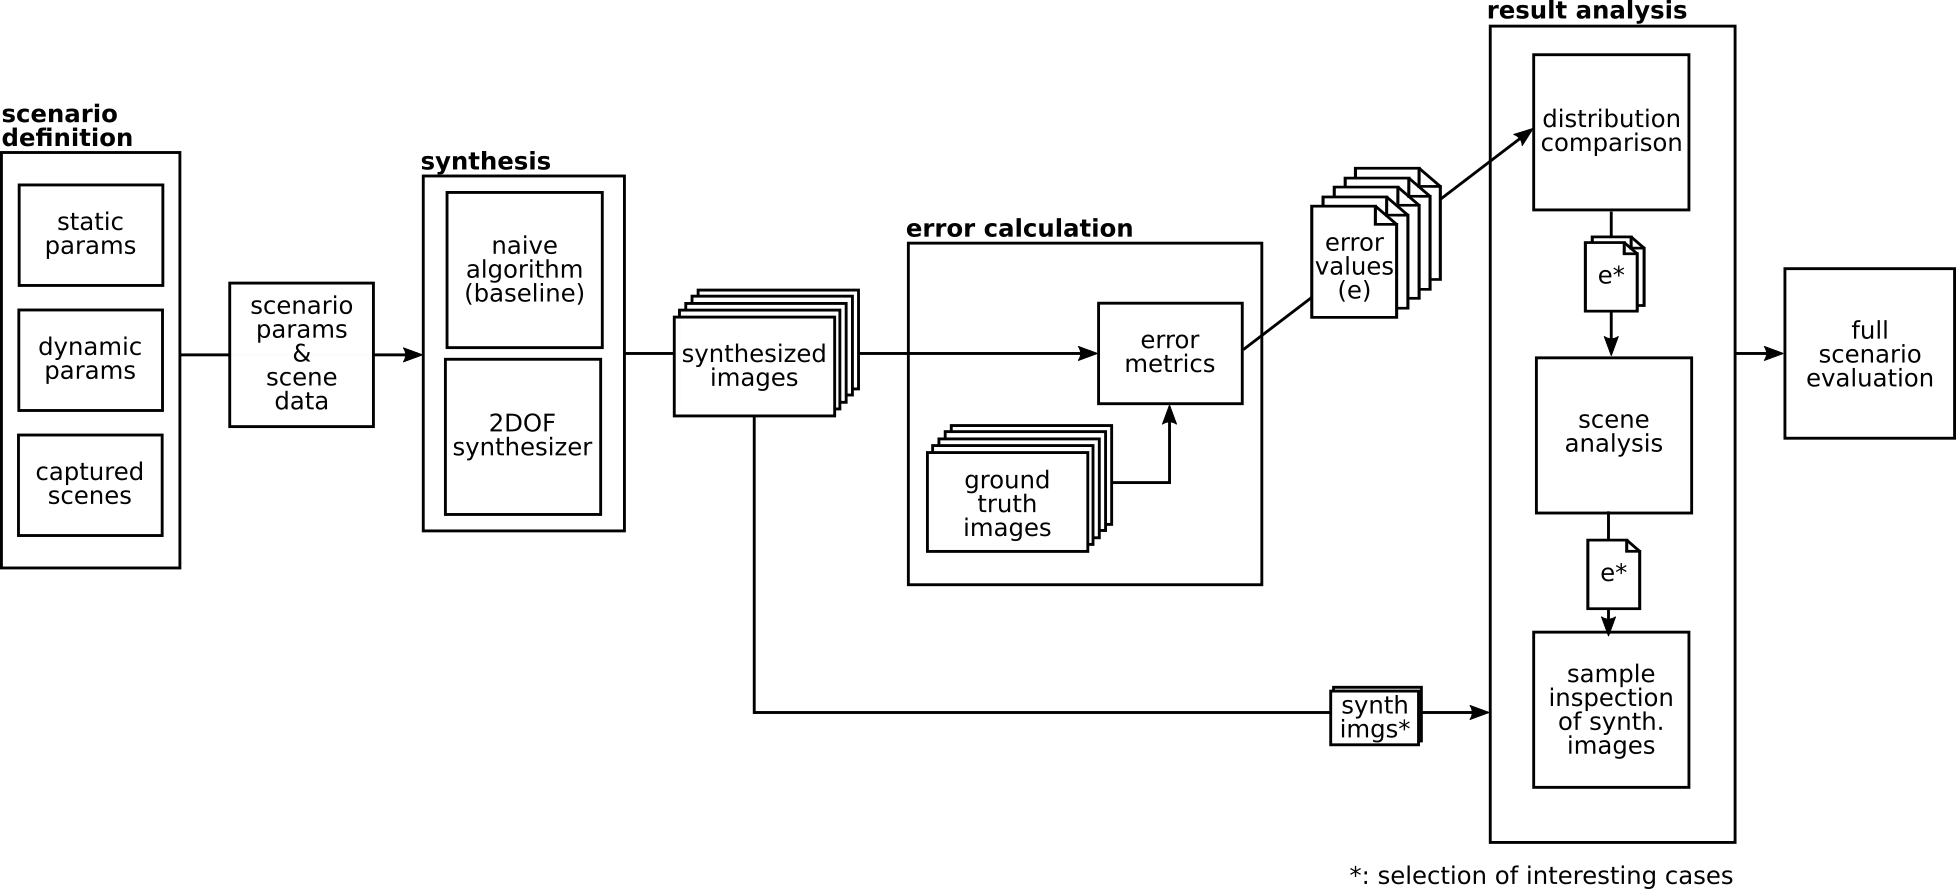
\includegraphics[width=\textwidth]{04/eval_methodology.png}
		\caption{Methodology for the evaluation of a scenario}
		\label{fig:eval-methodology}
\end{figure}

\subsubsection{Scenario Definition}
A scenario is defined by the parameter that it tests, the static parameters that are used, and the scene where the data was captured. Although a scenario is designed to test a specific parameter, which then is ``dynamic'' (i.e.\ will be modified throughout the scenario), there might also be more dynamic parameters. For example, in a scenario for exploring viewpoint density, the blending type might also be modified to see what effect the viewpoint density has on regular and flow-based blending. The static parameters include for example the location of the synthesized viewpoints, or any other parameter that remains unchanged throughout the scenario. One other defining factor of a scenario is the scene data that the scenario is tested on. Although the scene is part of the parameters (the external parameters, to be exact), it merits particular mention, as it contains the actual image data that is used for synthesis. This data, along with the other parameters defined in the scenario, are then passed on to the synthesis step.

%First, a scenario must be defined that illustrates the parameter that should be examined. This includes determining which of the parameters should be static, and which should be dynamic. There are two dynamic parameters at maximum, one to be examined, and one to increase the significance of the results. Adding more dynamic parameters per scenario would allow for a more definitive evaluation, but is outside of the scope of this thesis.

%The set of parameters (whether static or dynamic) contains the choice of scene in which to synthesize the images. The scene is defined by its captured viewpoints, metadata, and radius, which are all passed on to the synthesis step along with the other parameters defined for the scenario.

\subsubsection{Synthesis}
The synthesis step consists of two parts: the 2DoF synthesis presented in Chapter~\ref{chap:implementation} using either flow-based blending or regular blending depending on the scenario parameters, and a baseline synthesis using a naive algorithm.
The naive algorithm consists of simply selecting the nearest neighbor viewpoint based on euclidean distance. The input parameters are the same for both algorithms and both results are passed on to error calculation.
The results of the naive algorithm serve as a baseline comparison to verify whether the developed 2DoF algorithm is an improvement to a naive approach. If either the regular or the flow-based blending generally performed worse than the naive algorithm, this would be an indication of a substantial flaw in the approach.

\subsubsection{Error Calculation}
There are many properties that a synthesis algorithm can be evaluated for, for example performance, visual acceptability (based on user studies), number of artefacts, or distance from the ground truth. In this evaluation, mathematical
%In order to evaluate the synthesized images, it is necessary to define metrics with which to measure their accuracy. Since it is outside of the scope of this thesis to evaluate the quality of the results based on human perception, mathematical
error metrics are used to compare each result to its ground truth image.  Two different metrics are chosen based on different image features so that potential limitations of each metric can be compensated for by the other. However, it must be taken into account that neither are perfect for the task of measuring accuracy on 360\degree synthesized images, so their validity should always be taken with a grain of salt. 

\paragraph{L1 error on RGB}
The first metric is the L1 error calculated on the ground truth and result images in RGB color space. This is a simple error metric that calculates the mean absolute difference of the RGB values and therefore indicates the mean accuracy of each pixel of the image. The RGB errors of each pixel are added together for the complete image and then divided by the number of pixels in the image. This results in an error value $e \in [0,3]$, since the maximum error per pixel is 3 for floating point RGB color values $\in [0,1]$.

The L1 error can also be visualized by calculating the absolute difference per pixel without averaging the values. Figure~\ref{fig:l1_example} shows an example visualization of the L1 error between two images. The visualization encodes areas of the image where there is a very large difference with a value closer to white and areas where there is no difference as black, which clearly highlights areas of the image that are problematic.

The L1 error is useful because it gives a rough estimation of how accurately each pixel is synthesized. The visualization indicates in which areas the synthesized image is inaccurate, which is helpful for classifying problems. However, a drawback of the L1 error is that it relies on color values, which means that images with large differences in pixel values will generally produce a higher error value than images with smaller differences in pixel values, even though the distortion and displacement may be the same.

\begin{figure}
\centering
    \hfill
    \begin{subfigure}[t]{0.3\textwidth}
            \centering
            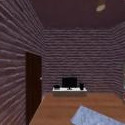
\includegraphics[width=0.9\textwidth]{04/l1_ex01.jpg}
            \caption{}
    \end{subfigure}%
    \hfill
    \begin{subfigure}[t]{0.3\textwidth}
            \centering
            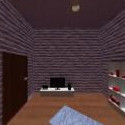
\includegraphics[width=0.9\textwidth]{04/l1_ex02.jpg}
            \caption{}
    \end{subfigure}
    \hfill
    \begin{subfigure}[t]{0.3\textwidth}
            \centering
            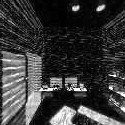
\includegraphics[width=0.9\textwidth]{04/l1_ex03.jpg}
            \caption{L1 error visualization of (a) and (b)}
    \end{subfigure}%
    \hfill
    \hfill
  \caption[Example visualization of L1 RGB error]{Example visualization of L1 RGB error. The RGB error values have been intensified so that they are more visible.} \label{fig:l1_example}
\end{figure}

As in the case of optical flow calculation, some adjustment must be made to adapt this metric for 360\degree images. Since the equirectangular projection is not equal-area, the areas towards the poles would intrinsically have higher weighting, since RGB L1 is calculated per pixel. To avoid this problem, the cube map projection is used, since it does not significantly distort the image. The average value is then calculated using the six faces of the cube, omitting the black background.

\paragraph{SSIM error on Grayscale}
The metric to complement the RGB L1 error is a variation of the the structural similarity index (SSIM) \cite{ssim}, which measures the \emph{structural similarity} between two images. Instead of comparing the images pixel by pixel, the SSIM uses the luminance, contrast and structure of the images for comparison. It compares these locally, i.e.\ it operates on smaller areas instead of the image as a whole. As a result, it is possible that the SSIM does not register small displacements in the scene if the objects are not distorted. However, the additional comparison with the RGB L1 error should mitigate this potential problem.

The SSIM metric in general, and the implementation used in the evaluation\footnote{skimage.metrics.structural\_similarity \cite{skimage}} return a value $\in [-1, 1]$ with 1 signifying an extremely similar image and -1 signifying a very different image. In order to more easily compare it with the RGB L1 error, the SSIM value is converted to an error value $ e \in [0,1]$, with 0 signifying an identical image (0 error) and 1 signifying a very different image.

The SSIM error is calculated on the grayscale image in cubemap representation. There is no need to use an RGB image, since it does not use the color values of an image. To avoid possible problems with distortion, the cubemap representation is again used.

\subsubsection{Result Analysis}
For each scenario evaluation, the number of results is made up of the dynamic parameters, the number of synthesized viewpoints, plus the baseline results. For each image, there are two error metrics to be considered.
%The number of parameters combined with the comparison to the baseline results and the use of two different error metrics results in a large number of error values.
In order to analyze these results effectively, it is necessary to break them down by creating different visualizations that highlight different attributes of the results.At first, an overview is created, from which interesting cases are selected and examined in more detail.

\paragraph{Distribution Comparison}
The first step of the analysis is a comparison of error value distribution. In order to compare all the error values of a scenario, they are plotted using a boxplot (Figure~\ref{fig:boxplot_example}). The different parameter combinations of the scenario are plotted on the y axis (e.g. viewpoint densities a, b, c) and the error distribution (i.e.\ the error values of all the synthesized viewpoints) is plotted on the x axis. The box plot shows the distribution of these values: the thick black line in the colored box is the median value (approx. 0.184 in Figure~\ref{fig:boxplot_example}), the colored ranges to the left and right of the median are the \ldots \todo{short description of a boxplot using the example}. Comparing the distribution of the results of a scenario gives a first general overview of the effect of the examined parameter from which interesting cases can be chosen for closer inspection.

\paragraph{Scene Analysis}
Based on the insights gained in the distribution comparison, several interesting cases are selected for closer analysis. These cases are examined by color coding the error values and assigning the colors to the positions in the scene. This puts the error values in context with the scene surroundings. Figure~\ref{fig:posmap_example} shows the synthesized points in the context of the scene, color coded by their error values. The maximum and minimum values of the points (also clearly visible in Figure~\ref{fig:boxplot_example}) are coded as dark red and dark blue, respectively. This visualization gives a more detailed overview over the values of the different points. In Figure~\ref{fig:posmap_example}, for example, the synthesized points near the right wall of the room have much better values than the row on the left side of the room. Using this information, it is possible to draw conclusions about the effect of the position of the synthesized viewpoint relative to the objects in the scene. This visualization also facilitates the selection of synthesized images that merit closer examination.

\begin{figure}
\centering
    \hfill
    \begin{subfigure}[c]{0.5\textwidth}
            \centering
            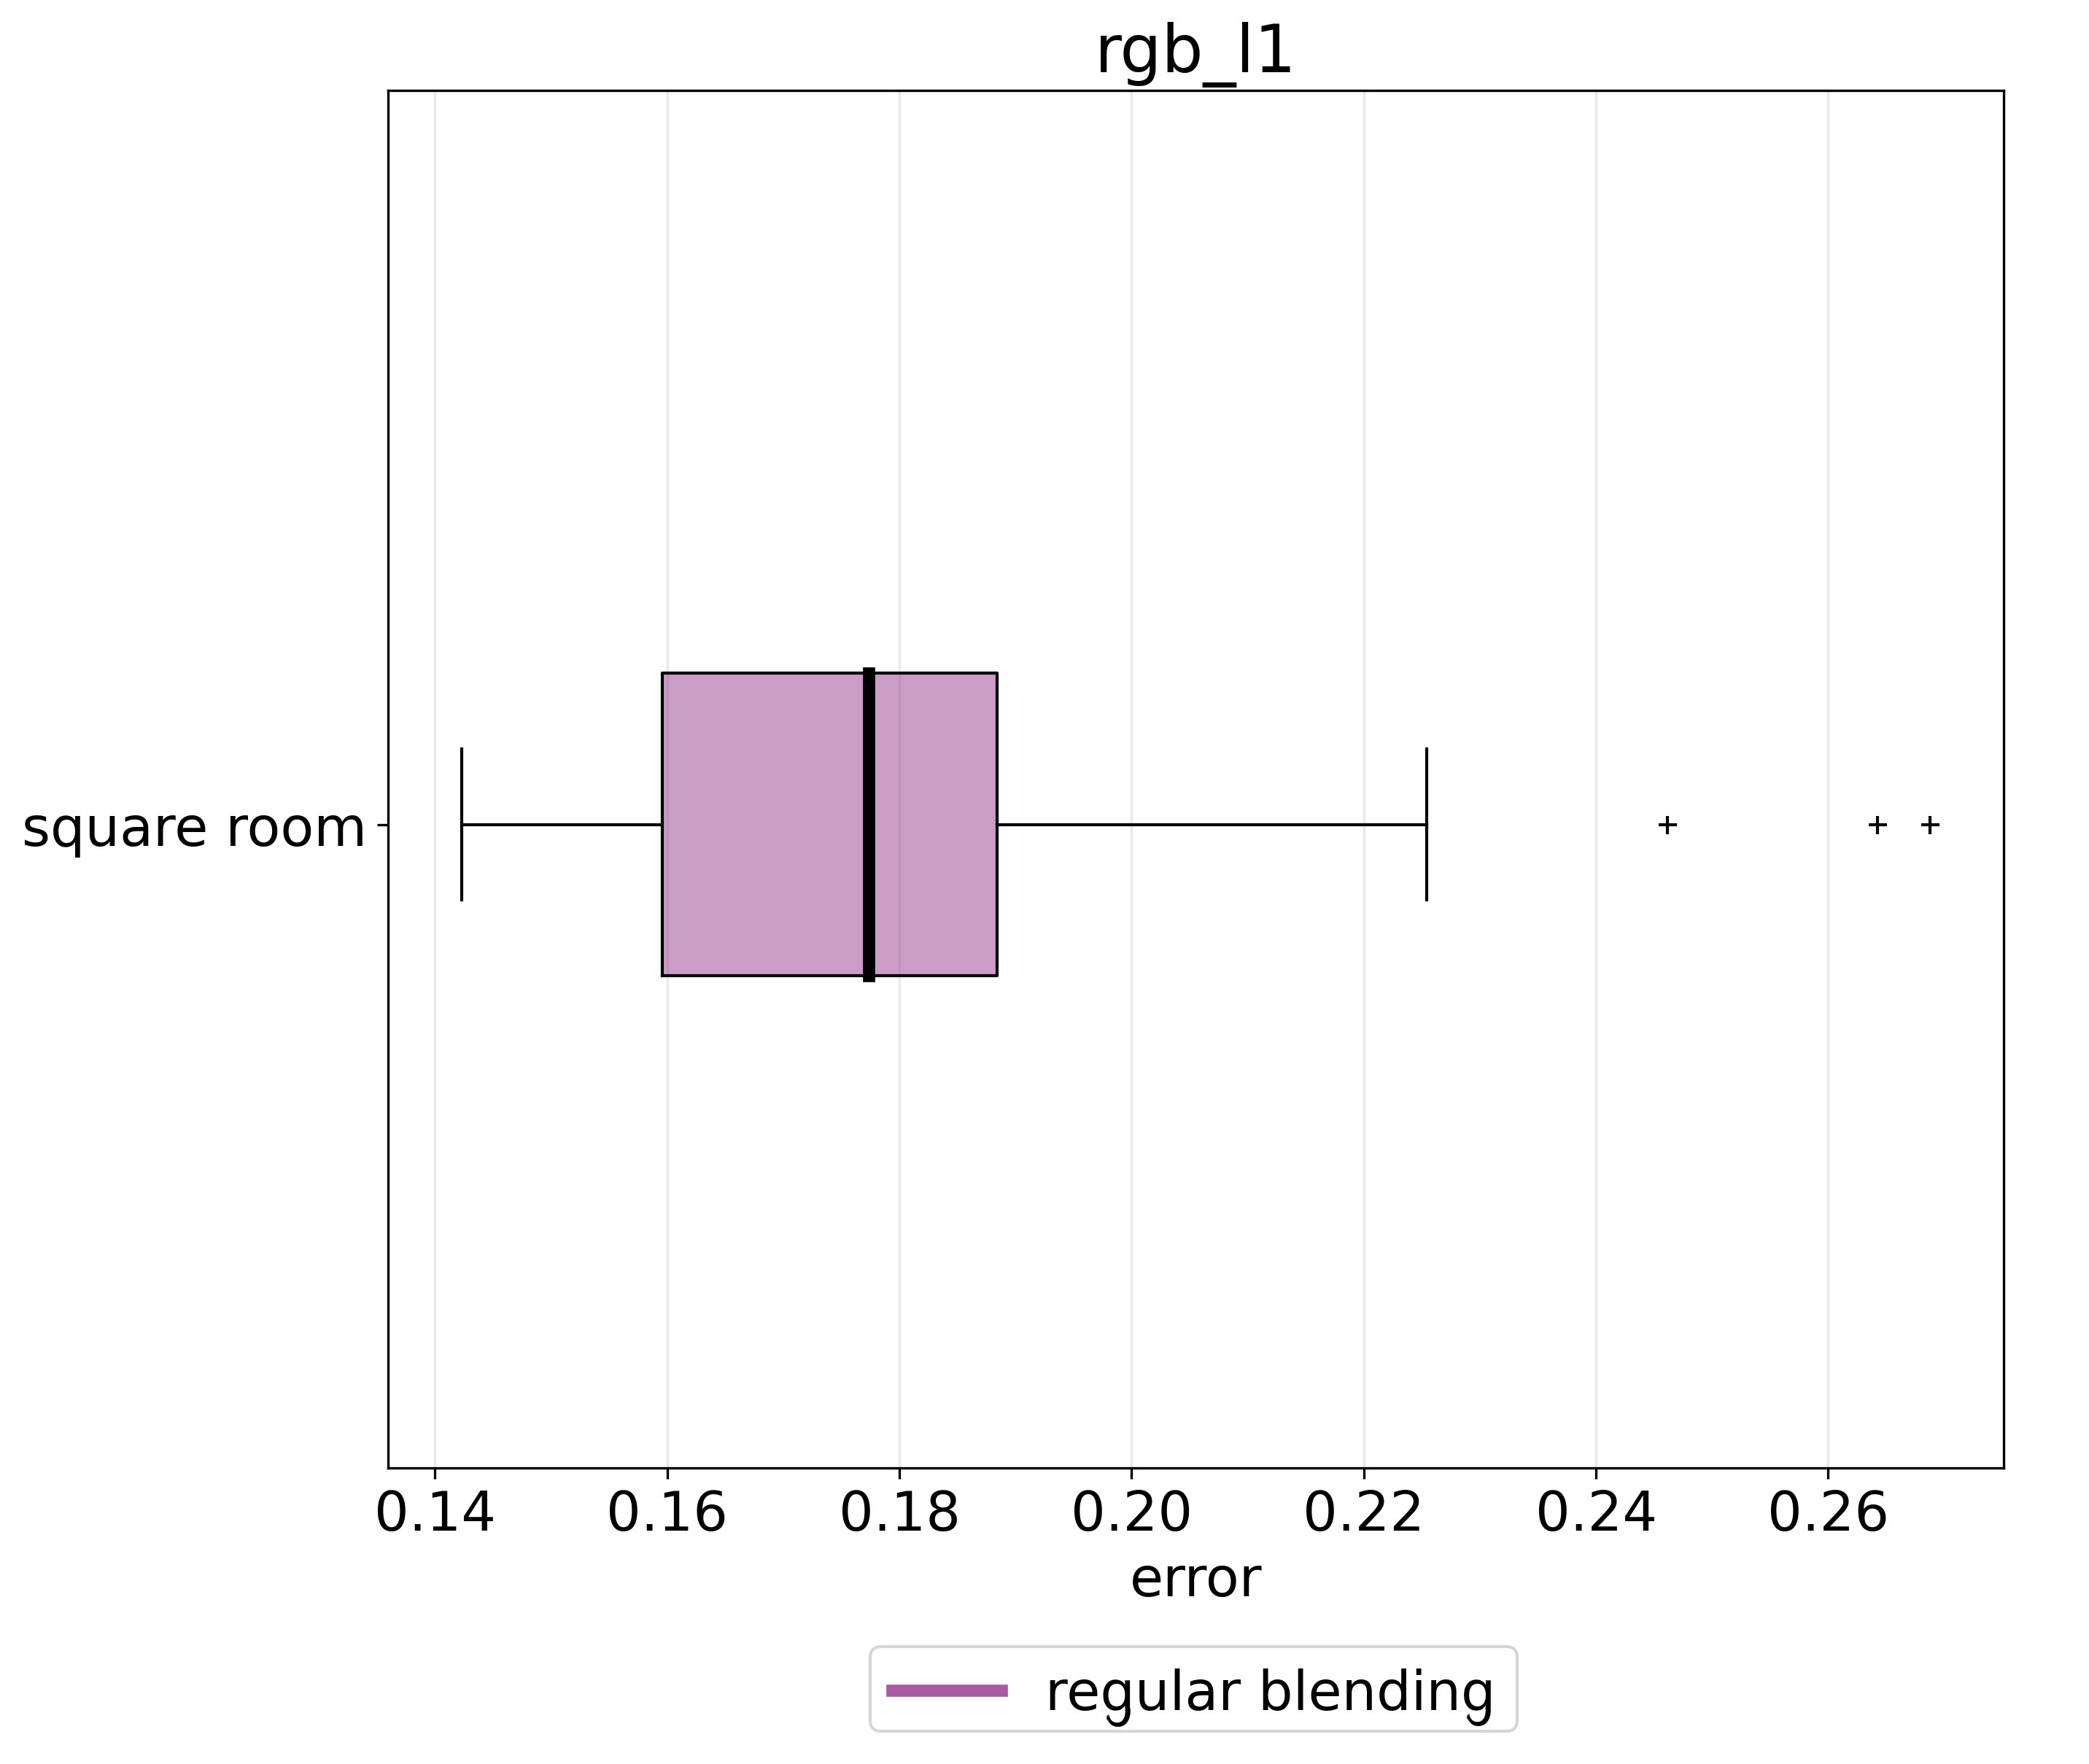
\includegraphics[height=6cm]{04/boxplot_example.jpg}
            \caption{Boxplot example for distribution comparison of the results of regular blending in the ``square room''} \label{fig:boxplot_example}
    \end{subfigure}%
    \hfill
    \begin{subfigure}[c]{0.5\textwidth}
            \centering
            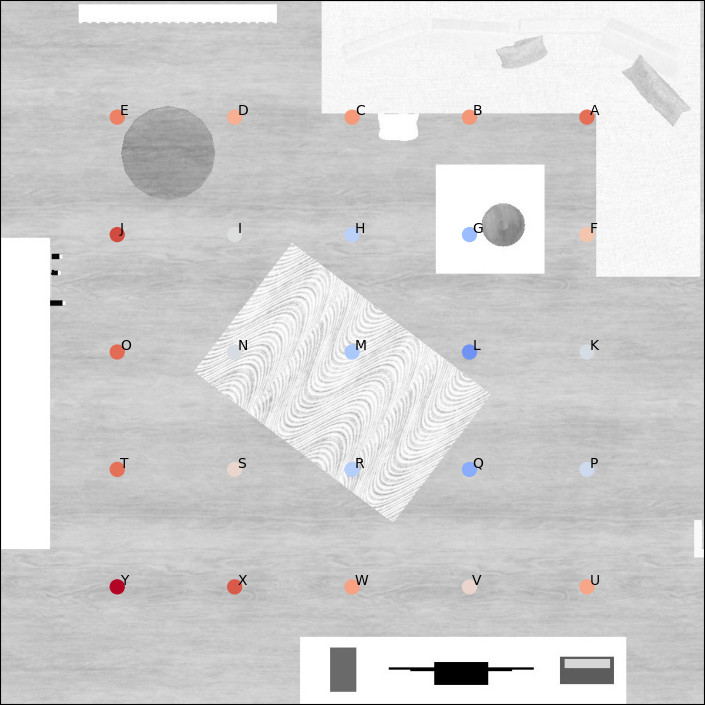
\includegraphics[height=6cm]{04/posmap_example.png}
            \caption{Visualization for scene analysis: The error values from the boxplot in (a) are mapped to colors at the positions of the viewpoints in the scene. Dark red represents the worst value (approx. 0.27) and dark blue the best value (approx. 0.145).} \label{fig:posmap_example}
    \end{subfigure}
    \hfill
  \caption[Different types of result visualizations for L1 error values]{Different types of result visualizations for L1 error values (``rgb\_l1'') for example results of regular blending in a scene}
\end{figure}

\paragraph{Sample Inspection}
In order to further understand the effects of the parameters on specific positions, some of the synthesized viewpoints from the scene analysis are examined manually by comparing the synthesized image to the ground truth image. The manual examination may also reveal information that the error metrics are unable to extract, such as specific types of artefacts.
\todo{insert an actual result here and explain how to read it!}

\section{Evaluation of Limits using Virtual Scenes} \label{sec:limit_eval}
The first step of the evaluation is to test the parameters of choice in a way that explores the limits of the algorithm. In order to have full control over the scene geometry, the objects within, and the positions of the captured and synthesized viewpoints, this limit evaluation is performed on virtual scenes created with the open source 3D animation software Blender \cite{blender}.

The parameters that will be explored are:
\begin{itemize}
  \item flow-based blending compared to regular blending
  \item the position of the synthesized points relative to the captured points
  \item the density of the captured viewpoints
  \item proxy-scene difference (how dissimilar is the scene geometry from the proxy sphere geometry)
\end{itemize}

Another factor that will be considered in all of the scenarios is the impact of the proximity and complexity of objects within the scene. However, since this is hard to parametrize, it will not be measured or explicitly tested.

%There is one internal parameter that is not specifically tested, but needs to be addressed, since it has a significant effect on the outcome of the flow-based blending: the optical flow algorithm. Fortunately, using virtual scenes generated with Blender can help mitigate mitigate this problem, since Blender has the capabilities to retrieve movement vectors from the geometry data, which can be used as optical flow.

\subsection{Data Acquisition and Featured Scenes} \label{subsec:data_acquisition}
In order to be able to test these scenarios, it is necessary to generate appropriate scenes. However, the manual capture of viewpoints as well as ground truth data can be very time-consuming. Furthermore, since locations need to be recorded either by hand, or calculated by a structure-from-motion algorithm or something similar, it is possible that the final locations are not perfectly accurate. In order to circumvent these problems, virtual scenes are used for the evaluation of limits. These scenes were created using the animation software Blender \cite{blender}. The position of the camera for each captured viewpoint was stored as a keyframe, so that the batch of viewpoints could be rendered like an animation. In order to automatically assign the viewpoints and the ground truth points to the keyframes, and write out the metadata, a blender script was implemented. This way the locations of the viewpoints are always perfectly accurate, and the ``capture'' of the viewpoints requires no manual effort, which means that it is possible to test a variety of different scenes and parameters with considerably less effort. In order to reduce viewpoint synthesis time, images with a resolution of 1000x500 were rendered for all of the scenes.

Three different scenes were modeled for testing: the \emph{checkersphere}, the \emph{square room} and the \emph{oblong room}.% and the \emph{oblong room II}.

\paragraph{Checkersphere}
The \emph{checkersphere} (Figure~\ref{fig:checkersphere}) is a perfect sphere with a diameter of approximately 2m. Its surface is covered with a checkerboard pattern with alternating colors of dark blue, dark red, and dark green. It represents a scene where the geometry of the scene is exactly the same as the proxy geometry. Although this kind of room is not likely to exist in reality, it serves as a good baseline, since the result of the reprojection should be very close to the ground truth. The checkerboard pattern was chosen so that distortions or inaccuracies are more visible.

\begin{figure}
\centering
    \hfill
    \begin{subfigure}[t]{0.7\textwidth}
            \centering
            \includegraphics[height=5cm]{04/checkersphere_overview.jpg}
            \caption{Latlong image from the center of the sphere}
    \end{subfigure}%
    \hfill
    \begin{subfigure}[t]{0.3\textwidth}
            \centering
            \includegraphics[height=5cm]{04/checkersphere_outside.jpg}
            \caption{View from the outside for reference}
    \end{subfigure}
    \hfill
  \caption{Overview of the ``checkersphere''}
  \label{fig:checkersphere}
\end{figure}

\paragraph{Square Room}
The \emph{square room} (Figure~\ref{fig:square_room}) is a room whose basic shape is a perfect cube with a side length of 3.5m. It contains an assortment of furniture\footnotemark: In one corner, there is an orange, L-shaped couch with dark blue and white cushions and a white marble couch table with a dark blue bowl on it, and several small, simple black and white pictures on the wall behind the couch. There is a blue and white rug in the middle of the room, and to the left of the couch are a round blue table, as well as a white radiator. On the wall next to the blue table is a white marble bookshelf containing several red books, as well as three wine bottles, and two decorational objects in green and purple. Across from the couch is a low marble cabinet with a black monitor, a black laptop and a black speaker on it. To the left of the cabinet is a wooden door with a gray handle. The walls are brick, painted a dark purple and there is a lamp with a white lampshade hanging from the middle of the ceiling.

\footnotetext{The furniture models used in the square room and the oblong room are adapted from \url{https://www.cgtrader.com/free-3d-models/interior/living-room/low-poly-interior-57731178-c955-4625-9e44-109c8eea5ee2}, by user ``miha29076'', and the textures are adapted from \url{https://www.poliigon.com/texture/plaster-17}, \url{ https://www.poliigon.com/texture/fabric-denim-003}, \url{https://www.poliigon.com/texture/wood-fine-dark-004}, and \url{https://www.poliigon.com/texture/interior-design-rug-starry-night-001}. \emph{All accessed last on September 23, 2020}}

The intention of using the square room is to allow approximate accuracy for the resampling step, while at the same time offering a more realistic indoor setting.

\begin{figure}
\centering
    \hfill
    \begin{subfigure}[b]{0.7\textwidth}
            \centering
            \includegraphics[height=5cm]{04/square_overview.jpg}
            \caption{Latlong image from the center of the room}
    \end{subfigure}%
    \hfill
    \begin{subfigure}[b]{0.3\textwidth}
            \centering
            \includegraphics[height=5cm]{04/square_top.jpg}
            \caption{Top view}
    \end{subfigure}
    \hfill
  \caption{Overview of the ``square room''}
  \label{fig:square_room}
\end{figure}

\paragraph{Oblong room}
The \emph{oblong room} (Figure~\ref{fig:oblong_room}) has a room size of approximately 5.5m x 3.5m and contains the same basic elements as the square room. It has the exact same furniture layout as the square room, except that some objects 

%The \emph{oblong room} (Figure~\ref{fig:oblong_room}) has a room size of approximately 5.5m x 3.5m and contains the same basic elements as the square room. There are two variations: the oblong room I, which has the exact same furniture layout as the square room, and the oblong room II, in which the furniture layout is modified. This modification can help in examining possible correlations of the scene geometry with the result. For example, the bookshelf is a fairly complex geometry that is at eye-level (as opposed to many other objects which are below eye-level). Placing it at different positions in the two scenes makes the correlation between the proximity to the bookshelf and the possibly worse results easier to recognize.

\begin{figure}
\centering
    \hfill
    \begin{subfigure}[b]{0.5\textwidth}
            \centering
            \includegraphics[height=4cm]{04/oblong_overview.jpg}
            \caption{``Oblong room''}
    \end{subfigure}%
    \hfill
    \begin{subfigure}[b]{0.5\textwidth}
            \centering
            \includegraphics[height=4cm]{04/oblong_top.jpg}
            \caption{Top view}
    \end{subfigure}
    \hfill
%
%    \hfill
%    \begin{subfigure}[b]{0.5\textwidth}
%            \centering
%            \includegraphics[height=4cm]{04/oblong2_overview.jpg}
%            \caption{``Oblong room II''}
%    \end{subfigure}%
%    \hfill
%    \begin{subfigure}[b]{0.5\textwidth}
%            \centering
%            \includegraphics[height=4cm]{04/oblong2_top.jpg}
%            \caption{Top view}
%    \end{subfigure}
%    \hfill
  \caption{Overview of the ``oblong room''}
  \label{fig:oblong_room}
\end{figure}

\subsection{Captured Viewpoints}
The viewpoint layout was chosen to be identical in all of the scenes. This means that all scenes contain 36 captured viewpoints, aligned in a regular grid of 6x6 viewpoints, with 60cm spacing. The grid of viewpoints is centered within the scene. This means that in the checkersphere (Figure~\ref{fig:vps_grid}a) and the square room (Figure~\ref{fig:vps_grid}b), the viewpoints cover approximately the complete scene, and in the oblong room, there is about a 1m area on each side of the grid that is not captured (Figure~\ref{fig:vps_grid}c and Figure~\ref{fig:vps_grid}d). It is necessary to take this difference in viewpoint coverage into account for the evaluation, since the viewpoints in the oblong room have a larger distance to two of the walls, which may have an effect on the accuracy of the results.

\begin{figure}
\centering
    \hfill
    \begin{subfigure}[b]{0.4\textwidth}
            \centering
            \includegraphics[width=0.9\textwidth]{04/vps_checkersphere.jpg}
            \caption{The captured viewpoints in the checkersphere}
    \end{subfigure}
    \hfill
    \begin{subfigure}[b]{0.4\textwidth}
            \centering
            \includegraphics[width=0.9\textwidth]{04/vps_square.jpg}
            \caption{The captured viewpoints in the square room}
    \end{subfigure}
    \hfill
    \hfill

    \hfill
    \begin{subfigure}[b]{0.4\textwidth}
            \centering
            \includegraphics[width=0.9\textwidth]{04/vps_oblong.jpg}
            \caption{The captured viewpoints in the oblong room}
    \end{subfigure}
%    \hfill
%    \begin{subfigure}[b]{0.4\textwidth}
%            \centering
%            \includegraphics[width=0.9\textwidth]{04/vps_oblong2.jpg}
%            \caption{The captured viewpoints in the oblong room II}
%    \end{subfigure}
%    \hfill
    \hfill
  \caption[The grid of captured viewpoints in each scene, including the proxy geometry]{The grid of captured viewpoints in each scene, including the proxy geometry (not to scale)} \label{fig:vps_grid}
\end{figure}

%, and the same number of synthesized viewpoints (25). Figure~\ref{fig:scene_setup} show how the points are set up in the different scenes. Using the same distances between viewpoints is important for comparing the accuracy (since larger distances may have an impact on the optical flow result), so the space occupied by the viewpoints is proportionally smaller in the oblong rooms (i.e. the viewpoints are not distributed in the entire room). This must be considered when evaluating the results.

\subsection{Synthesizing Ground Truth Optical Flow} \label{subsec:gt_of}
Using Blender to create virtual scenes not only facilitates capture, but also offers an alternative to calculating optical flow. As mentioned in Section~\ref{subsec:optical_flow}, most optical flow algorithms struggle with large displacements. The flow-based blending step in the 2DoF synthesis algorithm, however, assumes decent optical flow and there is no attempt to judge whether the optical flow calculation is feasible between two selected viewpoints. As a result, given the wrong circumstances (two viewpoints A and B that are far apart), the optical flow algorithm may fail, leading the flow-based blending to output undesirable results. The success of the optical flow algorithm is a prerequisite for the success of the 2DoF algorithm with flow-based blending.

However, the focus of this evaluation is not the accuracy of an arbitrary optical flow algorithm. In the best case, it would be possible to emulate ``perfect'' optical flow, thus decoupling the success of the optical flow from the success of the flow-based blending. While this is practically impossible for real scenes, virtual scenes theoretically contain all necessary information for retrieving ``ground truth'' optical flow. Blender, for example, is capable of ``rendering'' motion vectors using its vector speed render pass, which calculates the movement between points from one frame to the next in pixel space. The result is a motion vector field, which corresponds to the result of a ``classic'' optical flow algorithm. This, in the best case, ``ground truth'' optical flow was first presented by Butler et al.\ \cite{sintel} as a benchmark for optical flow algorithms.

Figure~\ref{fig:calc_vs_synth_flow} shows the improvement of the results of the 1DoF interpolation in the square room with three different distances of input viewpoints (2m, 60cm, 30cm). The interpolated viewpoint (orange) is always calculated at $\delta = 0.5$ between two captured viewpoints (blue). In this case, the interpolation algorithm is purely 1DoF, since only two viewpoints serve as input (i.e. no selection based on deviation angle, or resampling is necessary). The graphs show the improvement (decreasing error value) of the result with Blender flow compared to the result with Farneb\"ack optical flow.

\begin{figure}
		\centering
		\includegraphics[width=\textwidth]{04/blender_flow_improvement.png}
		\caption[Accuracy improvement with Blender flow versus Farneb\"ack flow]{Accuracy improvement with Blender flow versus Farneb\"ack flow: The y axis shows the improvement of the error metric when using Blender flow.}
		\label{fig:calc_vs_synth_flow}
\end{figure}

It is notable that using Blender's optical flow tends to improve the results, compared to Farneb\"ack's algorithm, but not in all cases. The reason for this is that the Blender optical flow (at least how it was calculated here), does not yield perfect ``ground truth'' optical flow, either. There are several possible reasons for this, mostly based on the fact that the process in Blender, like most optical flow algorithms, is designed for frame-to-frame use, and has been ``misused'' for distances that are infeasible for an actual animation. Nevertheless, no definitive explanation can be made at this point, since this would require in-depth understanding of Blender's vector speed render pass, which is outside of the scope of this thesis. Based on the results shown in Figure~\ref{fig:calc_vs_synth_flow}, and experience gained from testing both variants, the Blender optical flow is used for the limit evaluation, because, even though it is not perfect, it still seems to mostly yield better results than Scipy's implementation of Farneb\"ack's optical flow algorithm and as such decouples (to a degree) the success of the 2DoF synthesis with flow-based blending from the success of the optical flow algorithm.

%\begin{itemize}
%   \item points that are not visible because of perspective shift will not have a correspondence
%   \item distortion due to wide fov may have an effect on the results
%   \item even blender motion vectors are for frame to frame use, so it is possible, that large jumps do not work well because the blender algo can't handle it
%\end{itemize}

\subsection{Scenarios and Results}
Using the generated scenes and optical flow, as well as the parameters defined for this limit evaluation, it is now possible to design, test, and evaluate the scenarios. This section presents the scenes, viewpoint setups, and tested parameters used in each scenario, as well as the results of the tests, which are evaluated using distribution comparison, scene analysis, and sample inspection, as described in Section~\ref{sec:eval_methodology}. First the effect of the parameter on the regular blending results is examined, then the effect on the flow-based blending results is examined, and finally, the the results of the regular blending are compared to the results of the flow-based blending.

\subsubsection{The Effect of Different Scene Geometries}
The first parameter to be examined is the effect of different scenes on the accuracy of the results generated using regular blending and flow-based blending. A key factor of this scenario is how different the scenes are from the proxy geometry. The larger the difference, the more inaccurate the result of the resampling will be. There are two attributes of a scene that may have an influence on the result: the basic shape of the scene (e.g. sphere, cube, rectangular prism, or arbitrary polygon), and the objects within the scene. The different scenes presented in \ref{subsec:data_acquisition} mostly differ in their basic shape, however, the impact of the objects within the scene can be examined by scene analysis.

All of the virtual scenes are used (checkersphere, square room, oblong room). The arrangement of captured viewpoints in all the scenes is identical (6x6 grid with a spacing of 60cm), and 25 viewpoints are synthesized in each scene.
The synthesized points are near or in the center of each grid cell, since these are the areas where the deviation angles are the highest, and where the largest artefacts for the regular blending are expected to emerge. In the square and oblong rooms, the synthesized points are slightly offset from the center of each grid cell (Figure~\ref{fig:scene_setup}). The offset is important in order to test actual 2DoF synthesis, instead of just 1DoF interpolation, since synthesizing in the center of a grid cell could be done with only 1DoF interpolation (e.g. by interpolating by 0.5 between the top right to the bottom left captured viewpoint, as was done in Section~\ref{subsec:gt_of} for testing Blender optical flow). No offset was used in the checkersphere scene, since the checkersphere scene is expected to have excellent results for the regular blending (since the proxy geometry and scene geometry are identical). In this case it is more interesting to use one of the presumably best positions for the flow-based blending to see how well it holds up in comparison.

\begin{figure}
\centering
    \hfill
    \begin{subfigure}[b]{0.4\textwidth}
            \centering
            \includegraphics[width=\textwidth]{04/scenario_scene/sphere_points.jpg}
            \caption{The checkersphere}
    \end{subfigure}%
    \hfill
    \begin{subfigure}[b]{0.4\textwidth}
            \centering
            \includegraphics[width=\textwidth]{04/scenario_scene/square_points.jpg}
            \caption{The square room}
    \end{subfigure}
    \hfill
    \hfill

    \hfill
    \begin{subfigure}[b]{0.4\textwidth}
            \centering
            \includegraphics[width=\textwidth]{04/scenario_scene/oblong_points.jpg}
            \caption{The oblong room}
    \end{subfigure}%
    \hfill
%    \begin{subfigure}[b]{0.4\textwidth}
%            \centering
%            \includegraphics[width=\textwidth]{04/scenario_scene/oblong2_points.jpg}
%            \caption{The oblong room II}
%    \end{subfigure}
%    \hfill
    \hfill
  \caption[The captured and synthesized viewpoints in the different scenes]{The captured (blue) and synthesized (orange) viewpoints in the different scenes (scenes are not to scale)} \label{fig:scene_setup}
\end{figure}

\begin{figure}
\centering
    \hfill
    \begin{subfigure}[b]{0.45\textwidth}
            \centering
            \includegraphics[width=\textwidth]{04/scenario_scene/boxplot_regular.png}
            \caption{Regular blending}
    \end{subfigure}
    \hfill
    \begin{subfigure}[b]{0.45\textwidth}
            \centering
            \includegraphics[width=\textwidth]{04/scenario_scene/boxplot_flow.png}
            \caption{Flow-based blending}
    \end{subfigure}
    \hfill
  \caption{Comparing the distributions of the results in different scenes}
  \label{fig:scene_boxplot_split}
\end{figure}

\paragraph{Regular Blending Results}
Figure~\ref{fig:scene_boxplot_split}a shows the distributions of the error values for the regular blending results in the three scenes. The most striking feature of this distribution is that the checkersphere results show the highest error values for the L1 error, whereas they show the lowest values for the SSIM error. The reason for this are the error metrics: L1 errors on the RGB images of the checkersphere will produce a higher value in general because of the checkerboard texture. A small displacement of the checkerboard texture will in most cases generate a higher error for the RGB L1 metric than the same displacement at an arbitrary position in one of the rooms: the difference between a dark blue pixel of a dark checkerboard field, and a white pixel on a white checkerboard field is close to 1, whereas the difference between a dark brown pixel and a dark purple pixel (e.g. between the door and the wall in one of the rooms) will produce a lower error value, although the distortion or displacement may be identical. The SSIM metric, which does not take the color values of the pixels into account, produces a distribution that is much closer to the expected result: Since the proxy geometry is identical to the real geometry, the result of the resampling should be almost perfect. And in fact, when visually comparing the results of a synthesized viewpoint to the ground truth (Figure~\ref{fig:scene_checkersphere_Y}, page~\pageref{fig:scene_checkersphere_Y} of Appendix~\ref{imgs}), the only difference is a little bit of blurriness due to resampling. The L1 difference depicted in the right column of Figure~\ref{fig:scene_checkersphere_Y} shows how the blurriness caused the high L1 error.

The trend of the error metrics of the other two rooms is consistent. This is likely due to the fact that they use identical textures, so the RGB errors are comparable. The results however, are surprising: Instead of yielding better results because the proxy geometry is closer to the general geometry of the square room, the errors of the square room are generally higher than those of the oblong room. A closer scene analysis (Figure~\ref{fig:scene_regular_square_oblong}) shows the probable reason for this: The error values in the square room (Figure~\ref{fig:scene_regular_square_oblong}a) are particularly high near the bookshelf on the left side of the room. Comparing the synthesized images at location ``O'' (right in front of the bookshelf) for the two scenes (Figure~\ref{fig:scene_square_oblong_O}, page~\pageref{fig:scene_square_oblong_O} of Appendix~\ref{imgs}) confirms this impression: The bookshelf is so close to viewpoint O in the square room, that there are extreme inaccuracies in the synthesis due to large deviation angles. In the oblong room, the bookshelf is much further away, making the devation angles much smaller and the result more accurate. The larger net distance to the walls and some of the objects in the oblong room is the likely reason for the lower error results throughout the scene.
\todo{maybe mention D or A as well}

\begin{figure}
\centering
    \hfill
    \begin{subfigure}[b]{0.45\textwidth}
            \centering
            \includegraphics[width=\textwidth]{04/scenario_scene/01_square__regular.png}
            \caption{Results of regular blending in the square room}
    \end{subfigure}
    \hfill
    \begin{subfigure}[b]{0.45\textwidth}
            \centering
            \includegraphics[width=\textwidth]{04/scenario_scene/01_oblong__regular.png}
            \caption{Results of regular blending in the oblong room}
    \end{subfigure}
    \hfill
  \caption{Scene analysis of regular blending results in the square and oblong rooms} \label{fig:scene_regular_square_oblong}
\end{figure}

\paragraph{Flow-based Blending Results}
The results of the synthesis using flow-based blending in the different scenes (Figure~\ref{fig:scene_boxplot_split}b) show similar tendencies as the results of the regular blending, except in the case of the checkersphere: Where the SSIM error in the checkersphere scene was significantly lower than the other two, in the flow-based blending results, the SSIM error yields worse results than the oblong room, but still mostly better than the square room. The worse performance of the flow-based blending in the checkersphere is likely due to the fact that the flow-based blending introduces some inaccuracies, for example due to imperfect optical flow, or ray approximation.

In the other cases, the results of the flow-based blending mirror those of the regular blending: The results in the oblong room are better than those in the square room. Looking at the examples in Figure~\ref{fig:scene_square_oblong_O} (page~\pageref{fig:scene_square_oblong_O} of Appendix~\ref{imgs}) shows that, like in the case of the regular blending, this is due to the relative postion of the walls and objects to the points: the synthesis with flow-based blending also performs a lot better when there is no detailed object in close proximity. This is likely due to failing optical flow due to large displacements. In Figure~\ref{fig:scene_square_oblong_O} it is clearly visible that the 1DoF interpolation has had an effect on the image, since, for example, the normally straight lines of the books are warped (bottom face), but a comparison with the ground truth shows that they are warped in a way that bears no resemblance to the actual position.

\paragraph{Comparing Regular Blending to Flow-based Blending Results}
The distributions of the error values of both the regular blending (purple) and the flow-based blending (blue) are shown in Figure~\ref{fig:scenario_scene_boxplot}, as well as the error value distribution of the naive algorithm (orange) for comparison\footnotemark. The graph shows that the average results of the flow-based algorithm tend to be slightly better than the results of the regular blending, except in the case of the checkersphere, and that the results of the regular blending tend to be distinctly better than those of the naive algorithm. 
\footnotetext{The naive algorithm error values of the checkersphere were omitted because they were so much higher than the other values that the scale of the plot became too small.}

In the case of the checkersphere, where the proxy geometry is identical to the model geometry, the regular blending distinctly outperforms the flow-based blending. However, this is to be expected. The goal of the flow-based blending approach aims to improve problems due to the difference between the real and proxy geometries, and it introduces possible inaccuracies (optical flow, ray approximation) in order to do so. For this case, where the scene geometry is identical to the proxy geometry, it is superfluous.

For the square room and the oblong room, the net improvement of the flow-based blending versus the regular blending is shown in Figure~\ref{fig:scene_diff_square_oblong}. At a glance, it is clear that in all cases in the oblong room, and in all but one or two cases in the square room (depending on the metric) the flow-based blending improved the result. However, the L1 value range is larger in the oblong room than it is in the square room, which will most likely result in more visible improvements in the oblong room. Figure~\ref{fig:scene_square_best_worst} (page~\pageref{fig:scene_square_best_worst} of Appendix~\ref{imgs}) shows the best (N) and worst (L) viewpoints in the square scene.

\begin{figure}
\centering
    \hfill
    \begin{subfigure}[b]{0.45\textwidth}
            \centering
            \includegraphics[width=\textwidth]{04/scenario_scene/diff_square_regular-flow.png}
            \caption{}
    \end{subfigure}
    \hfill
    \begin{subfigure}[b]{0.45\textwidth}
            \centering
            \includegraphics[width=\textwidth]{04/scenario_scene/diff_oblong_regular-flow.png}
            \caption{}
    \end{subfigure}
    \hfill
  \caption[Improvement of flow-based blending results over regular blending results in the square and oblong rooms]{Improvement of flow-based blending results over regular blending results in the square and oblong rooms. The stars denote the best and worst cases} \label{fig:scene_diff_square_oblong}
\end{figure}


\paragraph{}
In summary, the results of the synthesis in the three different scenes indicate that the general shape of the scene has an impact on the accuracy of the results (comparing the checkersphere to the other two scenes). However, the impact of the general shape seems to have a much smaller influence compared to the impact of the details of the geometry and the proximity of complex objects to the synthesized viewpoint. Based on the results\ldots


%square room 6x6 C flow is markedly better than regular

\begin{figure}
		\centering
		\includegraphics[width=\textwidth]{04/scenario_scene/all_boxplot.png}
		\caption[The distribution of results in different scenes]{Comparing the distribution of the results in different scenes for the naive algorithm, regular blending, and flow-based blending}
		\label{fig:scenario_scene_boxplot}
\end{figure}


Figure~\ref{fig:scene_checkersphere_Y} (page~\pageref{fig:scene_checkersphere_Y} of Appendix~\ref{imgs}) shows the results of viewpoint Y in the checkersphere scene, which is the viewpoint with the largest error difference between the regular blending and the flow-blending result. Apart from a  The flow-based blending result is also close, however, due to possible errors in optical flow, and the ray approximation problem, the error value is higher. Even with these problems, the errors are hard to recognize visually (due to the resolution, but also due to the fact that they are not very severe). The higher error values of the flow-based blending are better visible in the L1 difference images in the right column.

An interesting observation when comparing the results of the checkersphere with the results of the other scenes (Figure~\ref{fig:scenario_scene_boxplot}) is that the checkersphere's L1 errors are higher than all the other scene's L1 errors, whereas the SSIM error, especially of the regular blending results, are very low.


\subsubsection{Effect of Viewpoint Density on Flow-based Blending and Regular Blending}
For this scenario, the square room is used, as the viewpoint grid covers the entire area of the room, which guarantees higher proximity to all the objects. Three different versions of the captured viewpoint grid are used: a 2x2 grid with a spacing of approximately 2m (Figure~\ref{fig:density_setup}a), the 6x6 grid with a spacing of approximately 60cm, as was used in the previous scenario (Figure~\ref{fig:density_setup}b), and a 12x12 grid with a spacing of approximately 30cm (Figure~\ref{fig:density_setup}c). The 2x2 grid was chosen since it is the minimal grid to cover the entire room, and the 12x12 grid was chosen, since it halves the distance of the 6x6 grid and retains the relative positioning of the captured viewpoints versus the synthesized viewpoints\todo{really?}.
%- want to be able to compare them to each other \ar same synthesized viewpoints with different densities \ar need controllable distances to the synthesized viewpoints

\begin{figure}
\centering
    \hfill
    \begin{subfigure}[t]{0.3\textwidth}
            \centering
            \includegraphics[width=0.9\textwidth]{04/scenario_density/2x2_points.jpg}
            \caption{A density of 4 viewpoints (2x2 grid)}
    \end{subfigure}
    \hfill
    \begin{subfigure}[t]{0.3\textwidth}
            \centering
            \includegraphics[width=0.9\textwidth]{04/scenario_density/6x6_points.jpg}
            \caption{A density of 36 viewpoints (6x6 grid)}
    \end{subfigure}
    \hfill
    \begin{subfigure}[t]{0.3\textwidth}
            \centering
            \includegraphics[width=0.9\textwidth]{04/scenario_density/12x12_points.jpg}
            \caption{A density of 144 viewpoints (12x12 grid)}
    \end{subfigure}
    \hfill
  \caption{The different captured viewpoint densities in the square room} \label{fig:density_setup}
\end{figure}

\paragraph{Effect of Viewpoint Density on Regular Blending Results}
Figure~\ref{fig:density_boxplot_split}a shows the general distribution of the results of the regular blending with varying viewpoint densities. Unsurprisingly, the accuracy of the results improves, the closer together the input viewpoints are. The reason for this is that the changes of perspective due to the change in position are smaller, the closer together the input viewpoints are. Since the distances are smaller, the deviation angles are also smaller, giving a more accurate result. 

\paragraph{Effect of Viewpoint Density on Flow-based Blending Results}
\begin{figure}
\centering
    \hfill
    \begin{subfigure}[b]{0.5\textwidth}
            \centering
            \includegraphics[width=\textwidth]{04/scenario_density/dens_boxplot_regular.png}
            \caption{Regular blending}
    \end{subfigure}%
    \hfill
    \begin{subfigure}[b]{0.5\textwidth}
            \centering
            \includegraphics[width=\textwidth]{04/scenario_density/dens_boxplot_flow.png}
            \caption{Flow-based blending}
    \end{subfigure}
    \hfill
  \caption{Comparing the distributions of the results in the square room with different densities}
  \label{fig:density_boxplot_split}
\end{figure}

\paragraph{Comparing Regular and Flow-based Blending}
Like in the previous scenario, the flow-based blending tends to have lower error values than the regular blending. The only setup where this is not the case is in the 2x2 L1 error, where the distribution is 

\begin{figure}
		\centering
		\includegraphics[width=\textwidth]{04/scenario_density/dens_boxplot.png}
		\caption[Comparing the distributions of the results in the square room with different densities of captured viewpoints]{Comparing the distributions of the results in the square room with different densities of captured viewpoints for the naive algorithm, regular blending, and flow-based blending}
		\label{fig:scenario_dens_boxplot}
\end{figure}

\begin{comment}
Hypothesis: higher density --> better results, but difference is larger for flow-based.

Hypothesis II: the effect of higher density is more marked near walls and corners

Test:
  - use square room and test 2x2, 6x6, 10x10
  - compare flow with flow, reg with flow, and reg with reg -> 3 graphs
\end{comment}

\subsubsection{Position of Synthesized Viewpoints Relative to Captured Viewpoints}
A feature that sets this approach apart from many other viewpoint synthesis algorithms using image correspondences is that it has two degrees of freedom, instead of only synthesizing images on a line between two viewpoints. Given the grid-like setup of the captured viewpoints, there are many cases in which the synthesized viewpoint is on a line between the captured viewpoints. In these cases, for some image areas (those whith the smallest deviation angles falling to the aligned captured viewpoints), the 1DoF interpolation will calculate the synthesized image at the correct location and there is no need for any reprojection. In all the cases where the location of the synthesized viewpoint is not on a line between two captured viewpoints, the 1DoF interpolation is followed by a reprojection. In the best case scenario, there would be no impact on the accuracy of the result, no matter whether the synthesized viewpoint is on a line between two viewpoints or not. However, due to possible reprojection errors based on the proxy-scene difference, as well as possible inaccuracies introduced by the approximation of non-viewpoint-plane rays (Section~\ref{subsec:2dof_flow-based} on page \pageref{subsec:2dof_flow-based}), it is probable that the position of the synthesized viewpoint relative to the captured viewpoints does have an effect on the result. In order to examine this, several experiments are set up that compare the accuracy of synthesized points in the optimal position (at the intersection between several captured viewpoints) to the accuracy of synthesized viewpoints non-optimal positions (not at the intersection between any captured viewpoints). The different scene setups are demonstrated in Figure~\ref{fig:offset_setup}.

\begin{figure}
\centering
    \hfill
    \begin{subfigure}[t]{0.5\textwidth}
            \centering
            \includegraphics[width=0.8\textwidth]{04/scenario_offset/square_points_centered.jpg}
            \caption{The grid of captured points (blue) with the locations of the synthesized points (orange) that lie exactly on the diagonal between four captured points (``centered'')}
    \end{subfigure}%
    \hfill
    \begin{subfigure}[t]{0.5\textwidth}
            \centering
            \includegraphics[width=0.8\textwidth]{04/scenario_offset/square_points_offset.jpg}
            \caption{In the second setup, the synthesized points are offset from the center to be approximately equal distant from all connecting lines between captured viewpoints (``offset'')}
    \end{subfigure}
    \hfill
    \hfill
  \caption[The different locations of the synthesized viewpoints]{The different locations of the synthesized viewpoints: centered vs offset (the circle around the scene represents the proxy sphere that was used)} \label{fig:offset_setup}
\end{figure}

These setups are tested on the ``square room'', where the pixel-based resampling works fairly well. 

%These setups are tested in two different rooms: the square room, and the oblong room I, in order to test whether the proxy-scene difference has an impact on the result.

\begin{figure}
		\centering
		\includegraphics[width=\textwidth]{04/scenario_offset/square_boxplot.png}
		\caption[The distribution of results with centered vs offset synthesized points]{Comparing the distribution of the results of the centered vs the offset synthesized points for flow-based blending and regular blending in the square room}
		\label{fig:scenario_offset_boxplot}
\end{figure}

The boxplot (Figure~\ref{fig:scenario_offset_boxplot}) shows the distribution of the results of the test on the square room. In both the flow-based blending performs slightly better than the regular blending. Looking at the different blending techniques separately, the average error values of the regular blending drop slightly in the offset setup for both the SSIM error and the L1 error, while they both rise slightly for the flow-based blending results.


flow-based rising is to be expected because of ray approximation

exact observations:
flow
- outer rows: top and bottom generally worsen for flow and offset (close to objects/walls, so problems are more extreme) left worsens, right improves but this could well be because of distance to objects increases/decreases
- middle points don't change too much 

regular:
- seems like only proximity to objects matters

\begin{figure}
\centering
    \hfill
    \begin{subfigure}[t]{0.4\textwidth}
            \centering
            \includegraphics[width=\textwidth]{04/scenario_offset/square_centered_regular.png}
            \caption{Centered points}
    \end{subfigure}%
    \hfill
    \begin{subfigure}[t]{0.4\textwidth}
            \centering
            \includegraphics[width=\textwidth]{04/scenario_offset/square_offset_regular.png}
            \caption{Offset points}
    \end{subfigure}
    \hfill
  \caption{Centered vs Offset points in the square room with regular blending} \label{fig:offset_vs_centered_regular}
\end{figure}

\begin{figure}
\centering
    \hfill
    \begin{subfigure}[t]{\textheight}
            \centering
            \includegraphics[height=0.25\textheight]{04/scenario_offset/square_centered_flow.png}
            \caption{}
    \end{subfigure}
    \hfill

    \hfill
    \begin{subfigure}[t]{\textheight}
            \centering
            \includegraphics[height=0.25\textheight]{04/scenario_offset/square_offset_flow.png}
            \caption{}
    \end{subfigure}
    \hfill
  \caption{} \label{fig:offset_vs_centered}
\end{figure}


\begin{verbatim}
- hypothesis: no big difference for regular blending, flow-based blending better if on axis

- test: compare results of offset points with centered points in square room (with different densities

- the worse the regular blending is, the worse the jumps/discontinuities at the borders will be for the flow-based(except on a direct line), since it is dependent on the regular blending
\end{verbatim}




\section{Proof-of-Concept Evaluation using Real Scenes} \label{sec:pof_eval}
%- captured using Ricoh Theta Z1 on a tripod

\section{Discussion} \label{sec:discussion}
%- latlong storage maybe not best option, since there is lots of redundancy
 However, since it is not possible to test with perfect optical flow, it remains uncertain whether even perfect optical flow could improve the accuracy of viewpoints that are extremely close to objects. Probably not, since there would be too high occlusions

\subsection{Limits}

limits of the evaluation:
\begin{itemize}
  \item metrics can show improvement, but not evaluate believability, plus, the improvement is not quantifiable
  \item pixel differences and ssim give no indication on human perception, so it is not possible to judge believability
  \item even though the results suggest it, cannot be sure that the metrics measured are significant/robust
  \item interactions between the parameters are not closely examined \ar possible that some parameter affects another in an unexpected way
  \item objects are not clearly classified/measured, so no quantifiable evaluation possible
  \item positional and rotational knowledge may be calculable by sfm algos, but we don't know what kind of impact accuracy of the metadata will have, since we are hand-recording metadata meticulously
  \item interactions between different parameters are not examined exhaustively, so no conclusive information
\end{itemize}

\begin{itemize}
  \item choice of gt points \ar fixed
  \item \ar offset of synth point from the line between two points (this would measure the effect of th 2DoF approximation
  \item distance from captured point (in the scenes, the gt points are always the furthest possible distance from all other points)
  \item optical flow accuracy in relation to the scene size etc
\end{itemize}
limitations also here?

Assuming radius accuracy does in fact make a slight assumption about the scene geometry. Using only the deviation angle will lead to ``spots'' where the distance is fairly large but the angle is zero. 

\subsection{Future Work}
\begin{itemize}
  \item ``guess'' an optimal radius without using viewpoint locations e.g. outside
  \item find a good weight function that balances deviation angle and distance appropriately
  \item use methods like SLAM in order to be independent of actually recording metadata by hand
  \item undistort extended cubemap e.g. by using methods like \cite{fov} which can undistort images up to 120\degree
  \item extend to 3D \ar input viewpoints could improve flow-based blending for areas towards the poles
  \item parallelization and offloading to gpu
  \item improve choice of $\delta$
  \item human perception evaluation with user study
  \item tradeoff between line consistency and perspective accuracy \ar would be interesting to introduce color constraints / optical flow smoothing, or other techniques to avoid discontinuities. this may come at the cost of accuracy
  \item use an HMD like in the paper for capture
\end{itemize}

